\documentclass[11pt,a4paper]{article}

% Packages
\usepackage[utf8]{inputenc}
\usepackage[T1]{fontenc}
\usepackage{lmodern}
\usepackage[margin=1in]{geometry}
\usepackage{graphicx}
\usepackage{hyperref}
\usepackage{xcolor}
\usepackage{listings}
\usepackage{booktabs}
\usepackage{longtable}
\usepackage{array}
\usepackage{fancyhdr}
\usepackage{titlesec}
\usepackage{tocloft}
\usepackage{parskip}
\usepackage{enumitem}
\usepackage{tikz}
\usepackage{fancyvrb}
\usepackage{mdframed}

% Colors
\definecolor{codebackground}{RGB}{245,245,245}
\definecolor{codeborder}{RGB}{200,200,200}
\definecolor{linkcolor}{RGB}{0,102,204}
\definecolor{sectioncolor}{RGB}{51,51,51}
\definecolor{accentcolor}{RGB}{0,128,128}

% Hyperref setup
\hypersetup{
    colorlinks=true,
    linkcolor=linkcolor,
    urlcolor=linkcolor,
    pdftitle={NFTmarket: A Complete Guide for Watermarking Experts},
    pdfauthor={NFTmarket}
}

% Code listing style
\lstset{
    backgroundcolor=\color{codebackground},
    basicstyle=\ttfamily\small,
    breaklines=true,
    frame=single,
    framerule=0.5pt,
    rulecolor=\color{codeborder},
    xleftmargin=0.5cm,
    xrightmargin=0.5cm,
    aboveskip=1em,
    belowskip=1em
}

% Custom mdframed environment for code blocks
\mdfdefinestyle{codeblock}{
    backgroundcolor=codebackground,
    linecolor=codeborder,
    linewidth=0.5pt,
    innerleftmargin=10pt,
    innerrightmargin=10pt,
    innertopmargin=10pt,
    innerbottommargin=10pt
}

% Section formatting
\titleformat{\section}
    {\normalfont\Large\bfseries\color{sectioncolor}}
    {\thesection}{1em}{}
\titleformat{\subsection}
    {\normalfont\large\bfseries\color{sectioncolor}}
    {\thesubsection}{1em}{}
\titleformat{\subsubsection}
    {\normalfont\normalsize\bfseries\color{sectioncolor}}
    {\thesubsubsection}{1em}{}

% Header/Footer
\pagestyle{fancy}
\fancyhf{}
\fancyhead[L]{\leftmark}
\fancyhead[R]{NFTmarket Guide}
\fancyfoot[C]{\thepage}
\renewcommand{\headrulewidth}{0.4pt}

% Custom commands
\newcommand{\keyword}[1]{\textbf{\textcolor{accentcolor}{#1}}}
\newcommand{\code}[1]{\texttt{#1}}

% Table column types
\newcolumntype{L}[1]{>{\raggedright\arraybackslash}p{#1}}
\newcolumntype{C}[1]{>{\centering\arraybackslash}p{#1}}

\begin{document}

% Title Page
\begin{titlepage}
    \centering
    \vspace*{2cm}

    {\Huge\bfseries NFTmarket\par}
    \vspace{0.5cm}
    {\LARGE A Complete Guide for Watermarking Experts\par}
    \vspace{1cm}
    {\Large\itshape How Invisible Watermarks Meet Blockchain Technology\\to Enable Copyright Trading\par}

    \vfill

    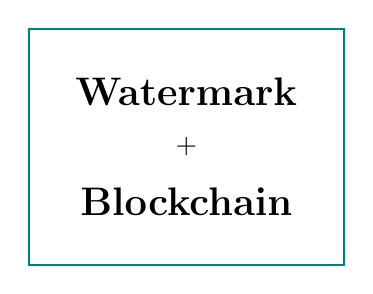
\begin{tikzpicture}
        \draw[thick, accentcolor] (0,0) -- (4,0) -- (4,3) -- (0,3) -- cycle;
        \node at (2,2.2) {\Large\bfseries Watermark};
        \node at (2,1.5) {+};
        \node at (2,0.8) {\Large\bfseries Blockchain};
    \end{tikzpicture}

    \vfill

    {\large NFTmarket Documentation\par}
    {\large \today\par}
\end{titlepage}

% Table of Contents
\tableofcontents
\newpage

% ============================================================================
\part{Foundation Concepts}
% ============================================================================

\section{The Problem We're Solving}

Traditional NFTs have a fundamental problem: \keyword{buying an NFT doesn't transfer any actual rights}.

When someone buys a typical NFT, they receive:
\begin{itemize}
    \item A database entry saying they ``own'' a token
    \item That's it
\end{itemize}

They do NOT receive:
\begin{itemize}
    \item Copyright
    \item The right to reproduce the image
    \item The right to make merchandise
    \item Any legal ownership of the artwork itself
\end{itemize}

Anyone can right-click, save the image, and use it however they want. The NFT buyer has nothing but a receipt.

\subsection{The Four Problems NFTmarket Solves}

\begin{enumerate}
    \item \textbf{NFTs don't convey ownership} -- Buying an NFT doesn't transfer copyright or usage rights
    \item \textbf{AI art has no provenance} -- Anyone can generate similar images; no way to prove who created first
    \item \textbf{Stolen art is rampant} -- Images are re-minted without consequences
    \item \textbf{Physical art lacks accessible authentication} -- Expensive gallery systems, easily forged certificates
\end{enumerate}

\subsection{The Solution}

NFTmarket combines \keyword{invisible watermarking} + \keyword{NFT minting} + \keyword{legal licensing} into a single transaction.

The watermark embeds the creator's identity directly into the pixels. The blockchain provides an immutable timestamp and ownership record. The license agreement defines exactly what rights are being sold.

\textbf{This is where your watermarking expertise becomes essential.} The watermark is the bridge between the digital image and the blockchain record. Without it, there's no way to connect a JPEG floating around the internet back to its token.

\newpage
\section{Blockchain Fundamentals}

Before we can understand NFTs, we need to understand what they live on: a blockchain.

\subsection{What Is a Blockchain?}

A blockchain is a \keyword{distributed database} replicated across thousands of computers worldwide. Every participant has an identical copy of all the data.

\begin{table}[h]
\centering
\begin{tabular}{@{}L{6cm}L{6cm}@{}}
\toprule
\textbf{Traditional Database} & \textbf{Blockchain} \\
\midrule
Runs on one company's servers & Runs on thousands of independent computers \\
Company controls it & No single party controls it \\
Company can modify data & Data is immutable once written \\
Trust the company & Trust the math \\
\bottomrule
\end{tabular}
\caption{Traditional Database vs Blockchain}
\end{table}

\subsection{Key Properties}

\textbf{Immutability}: Once data is written, it cannot be changed. Every ``block'' of transactions is cryptographically linked to the previous block. Changing old data would require re-computing every subsequent block, which is computationally infeasible.

\textbf{Transparency}: Everyone can see every transaction. The entire history of the database is public.

\textbf{Timestamps}: Each block has a timestamp that cannot be forged. You can prove exactly when something was recorded.

\textbf{No Central Authority}: No company, government, or individual controls the blockchain. It's maintained by a decentralized network of participants.

\subsection{Why This Matters for Art}

For the first time, we have a public, permanent, tamper-proof record of:
\begin{itemize}
    \item Who created something (and when)
    \item Who currently owns it
    \item Every transfer of ownership in between
\end{itemize}

This is the \keyword{provenance chain} -- the unbroken history from creation to the current owner.

\newpage
\section{What Is an NFT?}

An NFT (Non-Fungible Token) is surprisingly simple. It's just a \keyword{row in a database}.

\begin{mdframed}[style=codeblock]
\begin{verbatim}
Smart Contract Database
├── Token #0 → owned by 0xAlice
├── Token #1 → owned by 0xBob
├── Token #2 → owned by 0xAlice
└── Token #3 → owned by 0xCharlie
\end{verbatim}
\end{mdframed}

That's literally it. An NFT is an entry in a database that says ``token X is owned by address Y.''

\subsection{What ``Non-Fungible'' Means}

\textbf{Non-fungible means non-interchangeable} -- each token has a unique identity.

\begin{itemize}
    \item \textbf{Fungible:} One dollar bill equals any other dollar bill (interchangeable)
    \item \textbf{Non-Fungible:} Token \#0 $\neq$ Token \#1 (each is unique)
\end{itemize}

Two NFTs can have the same market price. ``Non-fungible'' just means they're tracked individually and can't be swapped blindly.

\subsection{What the NFT Points To}

The NFT itself doesn't contain the image. Storing images on the blockchain is prohibitively expensive.

Instead, the NFT contains a \textbf{pointer} (a URI) to where the image and metadata are stored:

\begin{mdframed}[style=codeblock]
\begin{verbatim}
Token #123
    → tokenURI: "ar://abc123..."  (Arweave permanent storage)
        → image: "ipfs://Qm..."   (IPFS decentralized storage)
        → name: "My Artwork"
        → description: "..."
\end{verbatim}
\end{mdframed}

\textbf{The ownership lives on the blockchain. The data lives off-chain but is verifiable.}

\subsection{The Standard Interface (ERC-721)}

All NFT contracts implement the same standard functions:

\begin{itemize}
    \item \code{ownerOf(tokenId)} -- Who owns this token?
    \item \code{transferFrom(from, to, id)} -- Transfer ownership
    \item \code{balanceOf(address)} -- How many tokens does this address own?
\end{itemize}

This standardization allows any marketplace or wallet to interact with any NFT.

\newpage
\section{Smart Contracts: The Database on the Blockchain}

A smart contract is a program that runs on the blockchain. Think of it as:

\textbf{Database} + \textbf{Code} + \textbf{Guaranteed Execution}

\begin{table}[h]
\centering
\begin{tabular}{@{}L{6cm}L{6cm}@{}}
\toprule
\textbf{Traditional App} & \textbf{Smart Contract} \\
\midrule
Database (like Postgres) & State variables (mappings, structs) \\
Backend code (like Node.js) & Solidity functions \\
Runs on your server & Runs on the blockchain \\
You control it & No one controls it \\
\bottomrule
\end{tabular}
\caption{Traditional App vs Smart Contract}
\end{table}

\subsection{What NFTmarket's Contract Stores}

The NFTmarketNFT smart contract stores:

\begin{mdframed}[style=codeblock]
\begin{verbatim}
struct TokenData {
    address creator;           // Original artist (never changes)
    address copyrightOwner;    // Current copyright holder
    LicenseType ownerLicense;  // Display, Commercial, or Transfer
    bytes32 imageHash;         // SHA-256 of the watermarked image
    bytes32 licenseHash;       // Hash of signed license agreement
    uint256 mintedAt;          // Block timestamp (immutable)
    string encryptedBlobUri;   // Where encrypted original is stored
}
\end{verbatim}
\end{mdframed}

\subsection{Key Functions}

\begin{table}[h]
\centering
\begin{tabular}{@{}ll@{}}
\toprule
\textbf{Function} & \textbf{What It Does} \\
\midrule
\code{mint()} & Create new NFT with license type \\
\code{list(tokenId, price, licenseType)} & List for sale \\
\code{buy(tokenId)} & Purchase (with payment) \\
\code{delist(tokenId)} & Remove listing \\
\code{ownerOf(tokenId)} & Query current owner \\
\code{getTokenData(tokenId)} & Query all metadata \\
\bottomrule
\end{tabular}
\caption{Smart Contract Key Functions}
\end{table}

\subsection{Why Contracts Are Powerful}

Once deployed, the code is \textbf{permanent and trustless}:
\begin{itemize}
    \item No one can change the rules after deployment
    \item The contract executes exactly as written
    \item Everyone can verify the code
    \item No company can shut it down or change behavior
\end{itemize}

\newpage
\section{Wallets: Your Digital Identity}

A wallet is how users interact with the blockchain. Despite the name, it doesn't ``store'' money -- it stores \keyword{cryptographic keys}.

\subsection{Public Key vs Private Key}

\begin{table}[h]
\centering
\begin{tabular}{@{}lll@{}}
\toprule
\textbf{Key Type} & \textbf{Purpose} & \textbf{Visibility} \\
\midrule
Public Key (Address) & Your identity, like an email & Share freely: \code{0x742d35Cc...} \\
Private Key & Proves you own the address & \textbf{NEVER share} \\
\bottomrule
\end{tabular}
\caption{Public vs Private Keys}
\end{table}

The address is derived mathematically from the private key. Anyone can send you things if they know your address. Only you can send things away (because only you have the private key).

\subsection{How Transactions Work}

Every blockchain transaction requires a \textbf{signature} from the sender's private key:

\begin{enumerate}
    \item User creates transaction: ``Send Token \#42 to 0xBob''
    \item User's wallet signs it with private key
    \item Transaction broadcast to network
    \item Network verifies signature matches address
    \item Transaction executed and recorded forever
\end{enumerate}

\subsection{Sign-In with Ethereum (SIWE)}

Instead of username/password, NFTmarket uses wallet signatures for authentication:

\begin{enumerate}
    \item Server sends a challenge message
    \item User signs it with their wallet
    \item Server verifies the signature
    \item User is authenticated
\end{enumerate}

No passwords to steal. No accounts to hack. Your identity is your cryptographic key.

% ============================================================================
\newpage
\part{The NFTmarket System}
% ============================================================================

\section{The NFTmarket Architecture}

NFTmarket consists of four independent components that communicate via API and blockchain:

\begin{mdframed}[style=codeblock]
\begin{verbatim}
┌─────────────────────────────────────────────────────────────────┐
│                        NFTmarket Platform                        │
├─────────────────────────────────────────────────────────────────┤
│                                                                  │
│  ┌──────────────┐  ┌──────────────┐  ┌──────────────────────┐  │
│  │   Frontend   │  │   Backend    │  │   Watermark Engine   │  │
│  │  (Flutter)   │  │  (Node.js)   │  │       (C++)          │  │
│  └──────────────┘  └──────────────┘  └──────────────────────┘  │
│                                                                  │
├─────────────────────────────────────────────────────────────────┤
│                                                                  │
│  ┌──────────────┐  ┌──────────────┐  ┌──────────────────────┐  │
│  │   Polygon    │  │  Cloud KMS   │  │        IPFS          │  │
│  │  Blockchain  │  │   (Keys)     │  │  (Decentralized)     │  │
│  └──────────────┘  └──────────────┘  └──────────────────────┘  │
│                                                                  │
└─────────────────────────────────────────────────────────────────┘
\end{verbatim}
\end{mdframed}

\subsection{The Services}

\begin{table}[h]
\centering
\begin{tabular}{@{}lll@{}}
\toprule
\textbf{Service} & \textbf{Port} & \textbf{Purpose} \\
\midrule
Flutter Web App & -- & User interface (browser-based) \\
Backend API & 3000 & Main application server \\
Wallet Service & 3001 & Key management and transaction signing \\
Hardhat Node & 8545 & Local blockchain for development \\
\bottomrule
\end{tabular}
\caption{NFTmarket Services}
\end{table}

\subsection{Data Flow}

\begin{mdframed}[style=codeblock]
\begin{verbatim}
User uploads image
       ↓
Backend: Apply watermark (wallet + tokenId)
       ↓
Backend: Encrypt original, upload preview to IPFS
       ↓
Backend: Upload metadata to Arweave (permanent)
       ↓
Backend: Store encrypted blob in Firebase Storage
       ↓
Wallet Service: Sign and submit mint transaction
       ↓
Blockchain: Record ownership, store hashes
       ↓
User: Owns NFT with embedded provenance
\end{verbatim}
\end{mdframed}

\subsection{Why a Separate Wallet Service?}

The Flutter web app \textbf{never touches private keys}. All signing happens in a separate microservice. This architecture:

\begin{itemize}
    \item Prevents key leakage through the frontend
    \item Allows different key management strategies
    \item Enables server-side signing for automated operations
    \item Keeps sensitive operations isolated
\end{itemize}

\newpage
\section{The License System: Selling Copyright}

This is where NFTmarket fundamentally differs from regular NFTs. Instead of just selling tokens, we sell \keyword{actual legal rights}.

\subsection{The Three License Types}

\begin{table}[h]
\centering
\begin{tabular}{@{}L{2.5cm}L{4cm}L{4cm}l@{}}
\toprule
\textbf{Type} & \textbf{What Buyer Gets} & \textbf{What Seller Keeps} & \textbf{Price} \\
\midrule
Display & Token + personal display rights & Copyright, commercial rights & \$1 \\
Commercial & Token + commercial usage rights & Copyright & \$5 \\
Transfer & Token + full copyright & Display rights only & \$10 \\
\bottomrule
\end{tabular}
\caption{License Types and Rights}
\end{table}

\subsection{License Hierarchy}

Rights form a strict hierarchy. \textbf{You cannot sell more rights than you have.}

\begin{mdframed}[style=codeblock]
\begin{verbatim}
Creator mints with Transfer → can sell Display, Commercial, or Transfer
Buyer gets Commercial      → can only resell Display or Commercial
Buyer gets Display         → can only resell Display
\end{verbatim}
\end{mdframed}

\subsection{What Each License Allows}

\textbf{Display License:}
\begin{itemize}
    \item Personal use only
    \item Can display in your home
    \item Can use as profile picture
    \item Cannot monetize
    \item Cannot make merchandise
    \item Cannot create derivatives
\end{itemize}

\textbf{Commercial License:}
\begin{itemize}
    \item Everything in Display, plus:
    \item Can monetize (sell prints, merchandise)
    \item Can use in commercial projects
    \item Can create derivatives
    \item Cannot transfer copyright to someone else
\end{itemize}

\textbf{Transfer License:}
\begin{itemize}
    \item Full copyright transfer
    \item Can do anything the original creator could do
    \item Can grant new licenses
    \item Previous owner retains only personal display rights
\end{itemize}

\subsection{Multi-License Marketplace}

A single token can have \textbf{up to three simultaneous listings} -- one for each license type:

\begin{mdframed}[style=codeblock]
\begin{verbatim}
Token #42 Listings:
├── Display:    0.5 ETH (personal use only)
├── Commercial: 2.0 ETH (can make merch)
└── Transfer:   10.0 ETH (full copyright)
\end{verbatim}
\end{mdframed}

Buyers choose their license level. The creator can earn from the same artwork multiple times at different price points.

\subsection{Bilateral Signatures}

Both buyer and seller sign the \textbf{exact same license agreement}:

\begin{mdframed}[style=codeblock]
\begin{verbatim}
┌─────────────┐         ┌─────────────┐
│   SELLER    │         │    BUYER    │
│             │         │             │
│ Signs:      │         │ Signs:      │
│ - tokenId   │         │ - tokenId   │
│ - price     │         │ - price     │
│ - license   │         │ - license   │
│ - hash      │         │ - hash      │
└─────────────┘         └─────────────┘
        │                       │
        └───────────┬───────────┘
                    ▼
         ┌─────────────────────┐
         │   BilateralAgreement │
         │   Event (on-chain)   │
         │                      │
         │  Both signatures     │
         │  recorded forever    │
         └─────────────────────┘
\end{verbatim}
\end{mdframed}

The license hash ensures both parties agreed to \textbf{exactly the same terms}. This creates a legally binding record on the blockchain.

\newpage
\section{The Minting Flow: From Image to NFT}

This is where watermarking integrates with the blockchain. Understanding this flow is essential.

\subsection{The Token ID Problem}

Here's a chicken-and-egg problem:
\begin{itemize}
    \item The watermark needs the token ID
    \item But the token ID is assigned during minting
    \item And minting requires the watermarked image first
\end{itemize}

\begin{mdframed}[style=codeblock]
\begin{verbatim}
Watermark needs tokenId
    ↓
Preview needs watermark
    ↓
Metadata needs preview URI
    ↓
Mint needs metadata URI
    ↓
Mint returns tokenId  ← too late!
\end{verbatim}
\end{mdframed}

\subsection{The Solution: Predict (or Reserve) the Token ID}

Token IDs are assigned sequentially. Before minting, we query \code{totalSupply()} and predict the next ID will be \code{currentSupply + 1}.

A more robust solution uses \textbf{reservation}:

\begin{mdframed}[style=codeblock]
\begin{verbatim}
Old flow (race condition risk):
  totalSupply() → predict ID → watermark → mint → hope IDs match

New flow (guaranteed):
  reserveTokenId() → get ID → watermark → mint(reservedId) → always match
\end{verbatim}
\end{mdframed}

\subsection{Complete Minting Flow}

\begin{enumerate}
    \item User uploads image
    \item Reserve tokenId on-chain (or predict it)
    \item \textbf{Apply watermark: embed (wallet + tokenId)}
    \item Calculate imageHash (SHA-256 of watermarked image)
    \item Generate preview (800$\times$800, FROM watermarked image)
    \item Encrypt watermarked original (AES-256)
    \item Upload preview to IPFS (public)
    \item Upload encrypted blob to Firebase Storage
    \item Create metadata JSON
    \item Upload metadata to Arweave (permanent)
    \item Mint NFT on Polygon (verify token ID matches)
    \item Store mapping in Firestore
\end{enumerate}

\subsection{What Gets Embedded in the Watermark}

\begin{mdframed}[style=codeblock]
\begin{verbatim}
Format: "0x742d35Cc6634C0532925a3b844Bc9e7595f8fE0E:123"
        └─────────────── wallet address ──────────────┘ └─ tokenId
\end{verbatim}
\end{mdframed}

Both pieces are needed:
\begin{itemize}
    \item \textbf{Wallet address}: Proves who created it
    \item \textbf{Token ID}: Identifies exactly which NFT it is
\end{itemize}

\subsection{What Gets Stored Where}

\begin{table}[h]
\centering
\begin{tabular}{@{}L{4cm}L{4cm}L{4cm}@{}}
\toprule
\textbf{Data} & \textbf{Location} & \textbf{Purpose} \\
\midrule
Token ownership & Blockchain & Source of truth \\
Mint timestamp & Blockchain & Immutable proof of priority \\
creator, copyrightOwner & Blockchain & Rights tracking \\
Preview (watermarked) & IPFS & Public display, traceable \\
Metadata JSON & Arweave & Permanent record \\
License documents & Arweave & Legal agreements \\
Encrypted original & Firebase Storage & Watermark detection \\
Encryption key & Cloud KMS & Controlled access \\
Watermark ID & Firestore + Metadata & Links image to token \\
\bottomrule
\end{tabular}
\caption{Data Storage Locations}
\end{table}

\subsection{Both Copies Are Watermarked}

\begin{table}[h]
\centering
\begin{tabular}{@{}lll@{}}
\toprule
\textbf{Image} & \textbf{Watermarked?} & \textbf{Where} \\
\midrule
Preview/thumbnail (800$\times$800) & \textbf{Yes} & IPFS (public) \\
Full-resolution original & \textbf{Yes} & Firebase Storage (encrypted) \\
\bottomrule
\end{tabular}
\caption{Watermarked Image Copies}
\end{table}

The preview is generated FROM the watermarked image. Screenshots of the preview carry the watermark and can be traced back to the token.

\newpage
\section{Buying and Selling Tokens}

\subsection{Listing Flow}

\begin{enumerate}
    \item \textbf{Seller:} Choose token, price, license type
    \item \textbf{Seller:} Read license agreement text
    \item \textbf{Seller:} Sign license agreement (EIP-712 typed data)
    \item \textbf{Seller:} Call \code{contract.list()} with signature
    \item \textbf{Contract:} Verify seller owns token
    \item \textbf{Contract:} Verify seller has rights to sell this license type
    \item \textbf{Contract:} Verify seller's signature
    \item \textbf{Contract:} Store listing (price, license, signature, expiry)
    \item \textbf{Contract:} Emit Listed event
\end{enumerate}

\subsection{Buying Flow}

\begin{enumerate}
    \item \textbf{Buyer:} Browse listings, find token
    \item \textbf{Buyer:} Read license agreement (same one seller signed)
    \item \textbf{Buyer:} Sign purchase acceptance (EIP-712)
    \item \textbf{Buyer:} Call \code{contract.buy()} with signature + payment
    \item \textbf{Contract:} Verify listing is active and not expired
    \item \textbf{Contract:} Verify payment is sufficient
    \item \textbf{Contract:} Verify buyer's signature
    \item \textbf{Contract:} Transfer license rights (based on license type)
    \item \textbf{Contract:} Distribute payment (97.5\% seller, 2.5\% platform)
    \item \textbf{Contract:} Transfer NFT ownership
    \item \textbf{Contract:} Emit Sold + BilateralAgreement events
\end{enumerate}

\subsection{License Rights Transfer}

\textbf{Display Sale:}
\begin{verbatim}
Before: Owner=Seller, Copyright=Seller, License=Display/Commercial/Transfer
After:  Owner=Buyer, Copyright=Seller, License=Display
\end{verbatim}

\textbf{Commercial Sale:}
\begin{verbatim}
Before: Owner=Seller, Copyright=Seller, License=Commercial/Transfer
After:  Owner=Buyer, Copyright=Seller, License=Commercial
\end{verbatim}

\textbf{Transfer Sale (Copyright Transfer):}
\begin{verbatim}
Before: Owner=Seller, Copyright=Seller, License=Transfer
After:  Owner=Buyer, Copyright=Buyer, License=Transfer
        Seller gets hasDisplayLicense[seller] = true (moral rights)
\end{verbatim}

\subsection{Payment Distribution}

\begin{table}[h]
\centering
\begin{tabular}{@{}lr@{}}
\toprule
\textbf{Recipient} & \textbf{Amount (1 ETH sale)} \\
\midrule
Platform (2.5\%) & 0.025 ETH \\
Seller (97.5\%) & 0.975 ETH \\
\bottomrule
\end{tabular}
\caption{Payment Distribution}
\end{table}

% ============================================================================
\newpage
\part{The Watermark-Blockchain Integration}
% ============================================================================

\section{How Watermarks Enable Copyright Trading}

\textbf{This is the crucial section.} Here's why your watermarking expertise is the foundation of the entire system.

\subsection{The Problem with Regular NFTs}

With a standard NFT:
\begin{enumerate}
    \item Someone right-clicks and saves your image
    \item They repost it, crop it, screenshot it, share it
    \item There is \textbf{zero connection} between that JPEG and your NFT
    \item You can't prove it's yours. They can't prove it's not.
\end{enumerate}

\subsection{The Solution: Embedded Identity}

With NFTmarket:
\begin{enumerate}
    \item The watermark embeds \code{wallet:tokenId} into the pixels
    \item Someone right-clicks and saves your image
    \item The watermark \textbf{travels with the copy}
    \item Screenshots, downloads, reposts -- all carry the watermark
    \item Anyone can extract the watermark and query the blockchain
    \item Immediate proof of which token, who created it, who owns rights
\end{enumerate}

\subsection{Why Both Wallet AND Token ID?}

The watermark must contain \textbf{both pieces}:

\begin{table}[h]
\centering
\begin{tabular}{@{}ll@{}}
\toprule
\textbf{Embedded Data} & \textbf{Why It's Needed} \\
\midrule
Wallet address & Proves who created it \\
Token ID & Identifies exactly which NFT \\
\bottomrule
\end{tabular}
\caption{Watermark Data Requirements}
\end{table}

With just the wallet: You know who made something, but they might have minted 100 NFTs. Which one?

With just the token ID: Token \#42 could exist on any of thousands of contracts. Which one?

Together: Unique identification across the entire ecosystem.

\subsection{The Verification Chain}

\begin{mdframed}[style=codeblock]
\begin{verbatim}
Suspicious Image (JPEG, screenshot, whatever)
       ↓
Extract watermark → get wallet + tokenId
       ↓
Query blockchain for that token
       ↓
Confirm creator matches wallet from watermark
       ↓
Check copyrightOwner → who has rights now?
       ↓
Check mint timestamp → who minted first?
\end{verbatim}
\end{mdframed}

\textbf{The watermark is the sole link between an image and its token.}

\newpage
\section{The Dual-Proof System}

NFTmarket uses two independent systems that serve different purposes:

\subsection{Layer 1: The Watermark (Embedded in Pixels)}

The watermark \textbf{identifies the token}. It's baked into the file and travels with any copy.

\begin{table}[h]
\centering
\begin{tabular}{@{}ll@{}}
\toprule
\textbf{Property} & \textbf{Description} \\
\midrule
Survives & Screenshots, downloads, JPEG compression, resizing \\
Can be extracted from & Any copy of the image \\
Contains & Creator wallet address + token ID \\
\bottomrule
\end{tabular}
\caption{Watermark Properties}
\end{table}

\subsection{Layer 2: The Blockchain (Immutable Record)}

The blockchain \textbf{proves ownership}. It's an external, permanent record.

\begin{table}[h]
\centering
\begin{tabular}{@{}ll@{}}
\toprule
\textbf{Data} & \textbf{Description} \\
\midrule
\code{creator} & Original artist (never changes) \\
\code{copyrightOwner} & Who holds current rights (changes on Transfer sales) \\
\code{mintedAt} & Block timestamp proving when created \\
\bottomrule
\end{tabular}
\caption{Blockchain Data}
\end{table}

\subsection{Why Both Layers Matter}

\begin{table}[h]
\centering
\begin{tabular}{@{}ll@{}}
\toprule
\textbf{Watermark} & \textbf{Blockchain} \\
\midrule
Identifies which token & Records who owns it \\
Survives image distortion & Immutable ownership history \\
Embedded in pixels & External record \\
The only link after transformation & Source of truth for rights \\
\bottomrule
\end{tabular}
\caption{Watermark vs Blockchain Roles}
\end{table}

If someone reposts your art without permission:

\begin{enumerate}
    \item Extract the watermark $\rightarrow$ get wallet + token ID
    \item Query the blockchain for that token $\rightarrow$ confirm creator, check current owner
    \item You have proof of which token it is and who owns the rights
\end{enumerate}

\newpage
\section{Protecting Original Images}

\subsection{Before Minting: Artist Responsibility}

\textbf{The unwatermarked original is a secret.} Whoever has it can mint it first.

There is \textbf{no automatic duplicate detection}. If someone gets your original before you mint:

\begin{enumerate}
    \item They upload it
    \item They mint it
    \item Their token has the earlier timestamp
    \item They ``own'' it according to the system
\end{enumerate}

\subsection{Best Practices for Artists}

\begin{table}[h]
\centering
\begin{tabular}{@{}L{6cm}L{6cm}@{}}
\toprule
\textbf{Do} & \textbf{Don't} \\
\midrule
Keep originals on encrypted storage & Post originals on social media \\
Mint first, share later & Send originals to ``collaborators'' \\
Share only watermarked versions & Store in cloud with weak passwords \\
\bottomrule
\end{tabular}
\caption{Artist Best Practices}
\end{table}

\subsection{The Blockchain Timestamp Is Your Proof}

Every mint is recorded with an immutable timestamp:

\begin{verbatim}
Token #42: Block 18,234,567 (January 15, 2025, 14:32:01 UTC)
Token #99: Block 18,300,000 (January 20, 2025, 09:15:44 UTC)
\end{verbatim}

\textbf{The earlier timestamp wins.} This cannot be forged.

If two people mint the same image, the one with the earlier blockchain timestamp has priority. The timestamp is proof that will hold up in any dispute.

\newpage
\section{Fraud Detection and Prevention}

\subsection{What the Watermark Protects Against}

If someone takes an \textbf{already-watermarked image} (screenshot, download, etc.) and tries to mint it:

\begin{enumerate}
    \item The original watermark is still embedded (original \code{wallet:tokenId})
    \item Detection via \code{/api/detect} reveals the original token
    \item The fraudster's token has a later timestamp
    \item Proof of fraud is clear
\end{enumerate}

\subsection{What the Watermark Does NOT Protect Against}

If someone obtains the \textbf{original unwatermarked image} before minting:

\begin{table}[h]
\centering
\begin{tabular}{@{}L{5cm}L{7cm}@{}}
\toprule
\textbf{Scenario} & \textbf{Outcome} \\
\midrule
Artist mints first, fraudster second & Artist has earlier timestamp = proof of fraud \\
Fraudster mints first with stolen original & Fraudster has earlier timestamp. Artist looks like fraud. \\
\bottomrule
\end{tabular}
\caption{Fraud Scenarios}
\end{table}

When a fraudster mints an original image, the system watermarks it with the \textbf{fraudster's} \code{wallet:tokenId}. There's no competing watermark to detect. The only evidence is timestamp comparison.

\subsection{If You Buy a Fraudulent Token}

\textbf{Bad luck.}

The buyer has no automatic recourse. Options:

\begin{enumerate}
    \item \textbf{Compare timestamps} -- Find the earlier token with the same image
    \item \textbf{Sue the seller} -- The seller's wallet address is on-chain
    \item \textbf{Social pressure} -- Public exposure of the fraudster's wallet
\end{enumerate}

The platform does not offer refunds or fraud protection. \textbf{Buyer beware.}

\subsection{Best Protection for Artists}

\textbf{Mint before your original leaks.} Once minted, the watermark and timestamp protect you. Before minting, there's no protection.

% ============================================================================
\newpage
\part{Technical Deep Dive}
% ============================================================================

\section{Storage Architecture}

\subsection{Where Everything Lives}

\begin{table}[h]
\centering
\begin{tabular}{@{}L{3cm}L{2.5cm}L{3.5cm}L{3cm}@{}}
\toprule
\textbf{Storage} & \textbf{Type} & \textbf{What It Stores} & \textbf{Durability} \\
\midrule
Blockchain (Polygon) & Decentralized & Ownership, timestamps, hashes & Permanent \\
Arweave & Permanent & Metadata, licenses & 200+ years \\
IPFS (Pinata) & Decentralized & Preview images & Requires pinning \\
Firebase Storage & Centralized & Encrypted originals & Depends on NFTmarket \\
Cloud KMS & Centralized & Encryption keys & Depends on NFTmarket \\
Firestore & Centralized & Token-to-key mappings & Depends on NFTmarket \\
\bottomrule
\end{tabular}
\caption{Storage Architecture Overview}
\end{table}

\subsection{Watermark-Relevant Storage}

\begin{table}[h]
\centering
\begin{tabular}{@{}L{4cm}L{4cm}L{4cm}@{}}
\toprule
\textbf{What} & \textbf{Where} & \textbf{Purpose} \\
\midrule
Watermarked preview & IPFS (public) & Display, contains watermark \\
Watermarked original & Firebase (encrypted) & Detection by authority \\
Encryption key & Cloud KMS & Controlled access \\
Watermark ID & Firestore & Links image to token \\
Mint timestamp & Blockchain & Immutable proof of priority \\
\bottomrule
\end{tabular}
\caption{Watermark-Related Storage}
\end{table}

\subsection{Why IPFS for Preview, Not for Encrypted Original?}

The encrypted blob is useless without the key. Since key management is centralized anyway, putting the blob on ``decentralized'' IPFS would be theater -- you still depend on NFTmarket to decrypt it.

Firebase Storage is simpler, cheaper, and honest about what's centralized.

\newpage
\section{The Central Point of Failure}

\textbf{This is the honest assessment.} The watermarking authority is essential and irreplaceable.

\subsection{If NFTmarket Disappears}

\begin{table}[h]
\centering
\begin{tabular}{@{}L{4cm}L{2cm}L{6cm}@{}}
\toprule
\textbf{Component} & \textbf{Status} & \textbf{Impact} \\
\midrule
Blockchain records & \textcolor{green!60!black}{\textbf{Survives}} & Ownership, timestamps intact \\
Arweave metadata & \textcolor{green!60!black}{\textbf{Survives}} & Name, description permanent \\
Arweave licenses & \textcolor{green!60!black}{\textbf{Survives}} & Legal agreements verifiable \\
IPFS previews & \textcolor{orange}{\textbf{At risk}} & Need someone to keep pinning \\
Encrypted originals & \textcolor{red}{\textbf{Lost}} & Cannot run detection \\
Encryption keys & \textcolor{red}{\textbf{Lost}} & Cannot decrypt originals \\
Watermark secret key & \textcolor{red}{\textbf{Lost}} & Cannot extract watermarks \\
Watermark extraction & \textcolor{red}{\textbf{Dead}} & Core value proposition dies \\
\bottomrule
\end{tabular}
\caption{Impact of NFTmarket Failure}
\end{table}

\subsection{Why There's No ``Publish the Spec'' Escape Hatch}

The watermark uses a secret key to:
\begin{itemize}
    \item Determine which frequency coefficients carry the data
    \item Generate the pseudorandom spreading sequence
    \item Scramble the embedded message
\end{itemize}

If this key were published:
\begin{itemize}
    \item Anyone could extract watermarks (fine)
    \item Anyone could \textbf{forge} watermarks (disaster)
    \item Anyone could \textbf{remove} watermarks (disaster)
\end{itemize}

\textbf{The secret key cannot be published.} This means watermark extraction will \textbf{always} require the authority.

\subsection{What Still Works Without the Authority}

Even if NFTmarket disappears:

\begin{enumerate}
    \item \textbf{``I own token \#123''} -- Query blockchain
    \item \textbf{``Token \#123 was minted on Jan 15, 2025''} -- Block timestamp
    \item \textbf{``The license agreement says X''} -- Fetch from Arweave, verify hash
    \item \textbf{``This exact file is token \#123''} -- Compare SHA-256 to on-chain imageHash
\end{enumerate}

\subsection{What Dies Without the Authority}

\begin{enumerate}
    \item \textbf{``This screenshot is from token \#123''} -- Can't extract watermark
    \item \textbf{``This JPEG is a copy of my NFT''} -- Can't trace transformed images
    \item \textbf{``This repost is my art''} -- No way to link image to token
\end{enumerate}

\textbf{The tokens don't become worthless} -- they become regular NFTs with nice legal documentation. But the watermark-based provenance, the thing that makes NFTmarket special, requires NFTmarket to keep operating.

\subsection{IPFS Failure vs NFTmarket Failure}

Two different failure modes:

\textbf{IPFS Failure (Pinata stops pinning):}
\begin{itemize}
    \item IPFS preview gone from network
    \item But any copy in the wild \textbf{still contains the watermark}
    \item Find any copy $\rightarrow$ extract watermark $\rightarrow$ restore provenance
    \item \textbf{The watermark saves you}
\end{itemize}

\textbf{NFTmarket Failure (company shuts down):}
\begin{itemize}
    \item Blockchain records safe
    \item Arweave permanent
    \item \textbf{Watermark extraction impossible} (secret key lost)
    \item Images become untraceable
\end{itemize}

The key difference:
\begin{itemize}
    \item IPFS fails $\rightarrow$ Watermark saves you (any copy works)
    \item NFTmarket fails $\rightarrow$ Watermark dies with it (secret key lost)
\end{itemize}

\newpage
\section{Copyright and Legal Reality}

\subsection{AI Art Cannot Be Copyrighted}

In the US (and increasingly elsewhere), copyright requires human authorship. The US Copyright Office has explicitly ruled that images generated by AI are not copyrightable.

\begin{table}[h]
\centering
\begin{tabular}{@{}L{8cm}l@{}}
\toprule
\textbf{Scenario} & \textbf{Copyrightable?} \\
\midrule
Human draws artwork & Yes \\
Human writes prompt, AI generates image & No \\
Human significantly modifies AI output & Maybe (only human parts) \\
\bottomrule
\end{tabular}
\caption{AI Art and Copyright}
\end{table}

\textbf{For AI art:} The ``Transfer'' license is selling something that doesn't legally exist. Both parties can agree to treat it as copyrighted, but courts may not enforce it.

\subsection{What the Watermark Actually Provides}

The watermark is \textbf{evidence}, not \textbf{enforcement}.

\begin{table}[h]
\centering
\begin{tabular}{@{}L{6cm}L{6cm}@{}}
\toprule
\textbf{It Proves} & \textbf{It Doesn't Provide} \\
\midrule
Which token an image came from & Automatic takedowns \\
Who minted first (timestamp) & Legal injunctions \\
Chain of custody & Damages recovery \\
That you own the NFT & Copyright (for AI art) \\
\bottomrule
\end{tabular}
\caption{What Watermarks Do and Don't Provide}
\end{table}

The watermark helps you prove your case. You still have to fight it yourself.

\subsection{The Opportunity for Physical Artists}

A painter could:

\begin{enumerate}
    \item Paint the artwork (copyright exists -- human creation)
    \item Photograph it (high quality digital capture)
    \item Mint a watermarked NFT with ``Transfer'' license
    \item Sell both together: physical painting + NFT
\end{enumerate}

The buyer now receives:
\begin{itemize}
    \item The physical painting (traditional sale)
    \item The NFT proving digital rights ownership
    \item Watermark protection against digital theft
    \item Signed bilateral agreement on-chain
\end{itemize}

This creates a legitimate market for reproduction rights that currently doesn't exist in the traditional art world.

\newpage
\section{Watermark Technical Details}

\subsection{The Watermarking API}

NFTmarket uses a cloud-hosted watermarking service.

\textbf{Endpoint: POST /watermark}

Request:
\begin{itemize}
    \item Header: \code{X-API-Key: <api-key>}
    \item Content-Type: \code{multipart/form-data}
    \item Body:
    \begin{itemize}
        \item \code{image} (required): PNG or JPG file
        \item \code{message} (required): Text to embed (\code{wallet:tokenId})
        \item \code{strength} (optional): 1-100, default 10
    \end{itemize}
\end{itemize}

Response (SSE stream):
\begin{verbatim}
data: {"progress":"Loading image...","percent":10}
data: {"progress":"Embedding watermark (1/5)","percent":24}
data: {"progress":"Compressing image...","percent":90}
data: {"complete":true,"downloadUrl":"/download/{jobId}"}
\end{verbatim}

\subsection{Watermark Properties}

\begin{table}[h]
\centering
\begin{tabular}{@{}L{4cm}L{2cm}L{6cm}@{}}
\toprule
\textbf{Transformation} & \textbf{Survives?} & \textbf{Notes} \\
\midrule
JPEG compression & Yes & Designed for this \\
PNG to JPEG conversion & Yes & Format-agnostic \\
Resizing/scaling & Yes & Multi-resolution embedding \\
Screenshots & Yes & Minimal transformation \\
Social media upload & Usually & Depends on compression level \\
Color adjustments & Mostly & Embedded in luminance channel \\
Print and scan & Sometimes & Most challenging attack \\
Cropping & Partial & Depends on how much removed \\
\bottomrule
\end{tabular}
\caption{Watermark Robustness}
\end{table}

\subsection{The Robustness Trade-off}

Watermarks balance three competing goals:

\begin{itemize}
    \item \textbf{Robustness} -- Survives transformations
    \item \textbf{Imperceptibility} -- Can't be seen
    \item \textbf{Capacity} -- How much data can be embedded
\end{itemize}

You can only optimize for two. NFTmarket prioritizes robustness and imperceptibility, embedding just enough data (wallet + tokenId) to establish provenance.

\newpage
\section{Future Directions: Zero-Knowledge Watermarks}

Can we prove a watermark exists \textbf{without revealing the secret key}?

\subsection{The Vision}

\begin{table}[h]
\centering
\begin{tabular}{@{}ll@{}}
\toprule
\textbf{Operation} & \textbf{Who Can Do It} \\
\midrule
Embed watermark & Authority only (has secret key) \\
Remove watermark & Authority only (knows where it is) \\
\textbf{Verify watermark} & \textbf{Anyone (via ZKP)} \\
\bottomrule
\end{tabular}
\caption{Zero-Knowledge Vision}
\end{table}

This would break the central point of failure for \textit{verification} while keeping \textit{embedding/removal} secure.

\subsection{How It Could Work}

\begin{enumerate}
    \item Authority publishes a \textbf{verification circuit} (the algorithm, not the key)
    \item At mint time, authority generates a \textbf{proof} for each image
    \item Proof stored on Arweave (permanent)
    \item Anyone can verify the proof against an image
    \item No secret key needed for verification
\end{enumerate}

\subsection{The Challenges}

\textbf{Circuit Complexity:} Watermark extraction involves DCT transforms, correlation with pseudorandom sequences, and thresholding -- expensive to encode as ZKP circuits.

\textbf{Transformation Handling:} ZKP proves ``this exact image has this watermark.'' But watermarks survive transformation. A screenshot won't match the proof for the original.

\textbf{New Minting Still Centralized:} ZKP helps verification, not embedding. The authority is still needed to mint.

\subsection{Current Status}

For MVP, we accept the central point of failure and document it honestly.

Future research directions:
\begin{enumerate}
    \item Asymmetric watermarking schemes (detection key $\neq$ embedding key)
    \item ZKP for exact-match verification (proofs on Arweave)
    \item TEE (Trusted Execution Environment) for transform-resistant verification
\end{enumerate}

The ``holy grail'' -- ZKP that handles arbitrary transformations -- is an open research problem.

% ============================================================================
\newpage
\section*{Summary: Key Takeaways}
\addcontentsline{toc}{section}{Summary: Key Takeaways}
% ============================================================================

\subsection*{For the Watermarking Expert}

\begin{enumerate}
    \item \textbf{Your watermark is the cornerstone.} Without it, there's no link between images and tokens.

    \item \textbf{The watermark embeds \code{wallet:tokenId}.} This uniquely identifies the token across the entire blockchain ecosystem.

    \item \textbf{Both preview and original are watermarked.} Screenshots of the preview can be traced.

    \item \textbf{The blockchain provides timestamps, not the watermark.} Priority disputes are resolved by block timestamps.

    \item \textbf{Extraction requires your secret key.} This is a central point of failure, but necessary for security.

    \item \textbf{The watermark survives transformation.} This is its key advantage over cryptographic hashes.
\end{enumerate}

\subsection*{What Makes This Different}

\begin{table}[h]
\centering
\begin{tabular}{@{}L{6cm}L{6cm}@{}}
\toprule
\textbf{Regular NFT} & \textbf{NFTmarket} \\
\midrule
Owns token, not image & Owns token + embedded proof \\
Screenshot = no connection & Screenshot = traceable \\
``Right-click save'' wins & Watermark survives \\
No legal agreement & Bilateral signed license \\
No copyright transfer & Explicit license types \\
\bottomrule
\end{tabular}
\caption{Regular NFT vs NFTmarket}
\end{table}

\subsection*{The Trade-offs}

\begin{table}[h]
\centering
\begin{tabular}{@{}L{6cm}L{6cm}@{}}
\toprule
\textbf{Benefit} & \textbf{Cost} \\
\midrule
Traceable provenance & Depends on watermarking authority \\
Clear license agreements & 2.5\% platform fee \\
Bilateral signatures & More complex UX \\
Copyright can be sold & Legal enforcement still required \\
\bottomrule
\end{tabular}
\caption{Benefits and Trade-offs}
\end{table}

\vfill

\begin{center}
\textit{This document was created to explain NFTmarket to a watermarking expert.}

\textit{For technical implementation details, see the individual documentation files in \code{/docs/}.}
\end{center}

\end{document}
